\begin{greek}
\chapter{Συλλογή σκουπιδιών πραγματικού χρόνου}\label{ch:rt}
Οι ταυτόχρονοι και αυξητικοί αλγόριθμοι συλλογής σκουπιδιών
που εξετάσαμε στο προηγούμενο κεφάλαιο προσπαθούν να μειώσουν
τους χρόνους παύσης που αντιλαμβάνεται ο τροποποιητής, είτε
με σπάσιμο του κύκλου συλλογής σε μικρά κβάντα χρόνου και την
παρεμβολή της εκτέλεσης του συλλέκτη στην εκτέλεση του τροποποιητή
για κάθε ένα από αυτά στον ίδιο επεξεργαστή, είτε με την ταυτόχρονη
εκτέλεση του συλλέκτη σε έναν διαφορετικό επεξεργαστή. Πολλοί
από τους αλγορίθμους αυτούς σχεδιάσθηκαν με στόχο την υποστήριξη
εφαρμογών πραγματικού χρόνου όπου οι παύσεις μεγάλης διάρκειας
έχουν ως αποτέλεσμα τη δραματική μείωση της επίδοσης. Παρότι
οι αρχικοί αυξητικοί και ταυτόχρονοι συλλέκτες κατηγοριοποιήθηκαν
ως πραγματικού χρόνου, αυτό είναι αληθές μόνο εάν τηρούνται
κάποιες αυστηρές προϋποθέσεις. Ωστόσο, όπως αντιλαμβανόμαστε
σήμερα τα συστήματα πραγματικού χρόνου, κανείς από τους αλγορίθμους
αυτούς δεν μπορεί να παρέχει ισχυρές εγγυήσεις προόδου στον
τροποποιητή. Η πρόοδος του τροποποιητή δεν μπορεί πλέον να
εγγυηθεί όταν ο τελευταίος πρέπει να αποκτήσει κάποιο κλείδωμα
(κατά την εκτέλεση κάποιου φράγματος εγγραφής ή ανάγνωσης για
παράδειγμα). Ακόμη χειρότερα, ένας διακοπτός αλγόριθμος χρονοδρομολόγησης
ενδέχεται τυχαία να δίνει μεγαλύτερη προτεραιότητα στη δρομολόγηση
των ταυτόχρονων νημάτων συλλεκτών. Η \textbf{συλλογή σκουπιδιών
πραγματικού χρόνου RTGC)} οφείλει να δικαιολογεί με ακρίβεια
τις παύσεις λειτουργίας των νημάτων τροποιητών, ενώ ταυτόχρονα
εξασφαλίζει τη μη υπέρβαση των χωρικών ορίων.

\section{Συστήματα πραγματικού χρόνου}
Τα \textbf{συστήματα πραγματικού χρόνου} επιβάλλουν λειτουργικές
προθεσμίες σε συγκεκριμένες εργασίες μιας εφαρμογής. Αυτά τα
συστήματα πραγματικού χρόνου θα πρέπει να αποκρίνονται σε
γεγονότα εισόδου εντός ενός καθορισμένου χρονικού παραθύρου.
Μια εργασία που αποτυχγάνει στην τήρηρη μιας προθεσμίας μπορεί
να υποβαθμίσει την υπηρεσία ή ακόμη χειρότερα να προκαλέσει
την πλήρη κατάρρευση του συστήματος. Συνεπώς, ένα σύστημα
πραγματικού χρόνου οφείλει να είναι ορθό όχι μόνο όσον αφορά
τη λογική της εφαρμογής, αλλά και όσον αφορά την αποκρισιμότητα
της σε γεγονότα πραγματικού χρόνου.

Ένα \textbf{απαλό σύστημα πραγματικού χρόνου} (όπως για παράδειγμα
η απεικόνιση βίντεο) μπορεί να ανεχτεί χαμένες προσθεσμίες εις
βάρος της ποιότητας της υπηρεσίας. Ενώ πολλές χαμένες προθεσμίες
θα έχουν ως αποτέλεσμα μη αποδεκτή ποιότητα υπηρεσίας, μια
συνηθισμένη χαμένη προθεσμία δεν την επηρεάζει πολύ. Ο Printezis
\cite{DBLP:journals/scp/Printezis06} προτείνει ένα απαλό στόχο
που προσδιορίζει ταυτόχρονα ένα μέγιστο χρόνο συλλογής, μία χρονική
σχισμή συγκεκριμένης διάρκειας και έναν αποδεκτό ρυθμό αποτυχίας.
Σε κάθε διάστημα εντός αυτής της χρονικής σχισμής, ο συλλέκτης
πρέπει να αποφύγει να χρησιμοποιήσει περισσότερο χρόνο από το
μέγιστο και όλες οι παραβιάσεις αυτού του στόχου πρέπει να είναι
εντός του αποδεκτού ρυθμού αποτυχίας. 

Ένας τέτοιος απαλός στόχος είναι ανεπαρκής για \textbf{σκληρά
συστήματα πραγματικού χρόνου} (όπως για παράδειγμα ο έλεγχος
ενός κινητήρα), όπου οι χαμένες προθεσμίες σημαίνουν την αποτυχία
του συστήματος. Ένα ορθώς σχεδιασμένο σκληρό σύστημα πραγματικού
χρόνου οφείλει να εξασφαλίζει την ικανοποίηση όλων των περιορισμών
πραγματικού χρόνου. Λαμβάνοντας υπόψη την παρουσία τέτοιων χρονικών
περιορισμών, είναι σημαντικό η αποκρισιμότητα της συλλογής
σκουπιδιών σε συστήματα πραγματικού χρόνου να μπορεί να χαρακτηρισθεί
με τέτοιο τρόπο ώστε να απεικονίζει τόσο τις ανάγκες της εφαρμογής
όσο και τη συμπεριφορά του συλλέκτη.

Η συνολική επίδοση ή ρυθμαπόδοση των συστημάτων πραγματικού χρόνου
είναι λιγότερο σημαντική από την \textbf{προβλεψιμότητα} της
επίδοσης. Η χρονική συμπεριφορά μιας εργασίας πραγματικού χρόνου
θα πρέπει να μπορεί να προσδιορισθεί είτε αναλυτικά κατά τη
σχεδίαση είτε εμπειρικά κατά την εκτέλεση ούτως ώστε ο χρόνος
απόκρισης της να είναι γνωστός εξαρχής (σε κάποιο αποδεκτό
βαθμό εμπιστοσύνης). Ο \textbf{χρόνος εκτέλεσης χειρότερης περίπτωσης}
μιας εργασίας είναι ο μέγιστος χρόνος που μπορεί να χρειαστεί
(αγνοώντας τυχόν επαναδρομολόγηση) για την απομονωμένη εκτέλεση
της εργασίας σε μια συγκεκριμένη πλατφόρμα υλικού. Συστήματα πραγματικού
χρόνου που υποστηρίζουν την ταυτόχρονη εκτέλεση πολλών εργασιών
πρέπει να δρομολογούν τις εργασίες με γνώμονα την ικανοποίηση
των χρονικών περιορισμών των τελευταίων. Η γνώση σχετικά με
την ικανοποίηση αυτών των περιορισμών απαιτεί την εκ των
προτέρων πραγματοποίηση \textbf{ανάλυσης δρομολόγησης}, υποθέτοντας
ένα συγκεκριμένο αλγόριθμο χρονοδρομολόγησης (συνήθως βασισμένο
σε προτεραιότητες).

Οι εφαρμογές πραγματικού χρόνου συχνά τρέχουν σε εξειδικευμένα
ενσωματωμένα συστήματα. Οι αλγόριθμοι αυξητικής συλλογής
σκουπιδιών είναι κατάλληλοι για χρήση σε ενσωματωμένα συστήματα
με μονοπύρηνο επεξεργαστή, ενώ οι αλγόριθμοι παράλληλης και
ταυτόχρονης συλλογής σκουπιδιών είναι πιο κατάλληλοι για χρήση
σε ενσωματωμένα συστήματα με πολυπύρηνο επεξεργαστή. Σε κάθε
περίπτωση πάντως, τα ενσωματωμένα συστήματα συχνά επιβάλλουν
στενότερους χωρικούς περιορισμούς σε σύγκριση με τις πλατφόρμες
γενικού σκοπού.

Για όλους τους παραπάνω λόγους, οι αλγόριθμοι συλλογής με
παύση του κόσμου, παράλληλης συλλογής ή ακόμη και ταυτόχρονης
συλλογής που επιβάλλει όμως μη προβλέψιμους χρόνους παύσης
δεν είναι κατάλληλοι για χρήση σε εφαρμογές πραγματικού
χρόνου. Ας θεωρήσουμε για παράδειγμα τη δρομολόγηση συλλογής
του σχήματος~\ref{fig:rt_1}, η οποία προκύπτει όταν η προσπάθεια
ανάκτησης μνήμης εξαρτάται από το συνολικό πλήθος και μέγεθος
των αντικειμένων που χρησιμοποιεί η εφαρμογή, τις διασυνδέσεις
μεταξύ των αντικειμένων αυτών καθώς και το βαθμό δυσκολίας ανάκτησης
αρκετής μνήμης για την ικανοποίηση μελλοντικών αιτημάτων. Δοθείσης
μιας τέτοιας δρομολόγησης, ο τροποποιητής δεν έχει κάποια εγγύηση
προβλέψιμης και βιώσιμης χρήσιμοποίησης του επεξεργαστή.

\begin{figure}
  \centering
  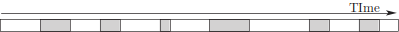
\includegraphics{figures/rt_1}
  \caption
    [Μη προβλέψιμη συχνότητα και διάρκεια εκτέλεσης συμβατικών
     συλλεκτών σκουπιδιών.]
    {Μη προβλέψιμη συχνότητα και διάρκεια εκτέλεσης συμβατικών
     συλλεκτών σκουπιδιών. Οι παύσεις λόγω συλλογής απεικονίζονται
     με γκρι χρώμα.}
  \label{fig:rt_1} 
\end{figure}

\section{Δρομολόγηση συλλογής πραγματικού χρόνου}
Ο χρόνος και ο τρόπος πυροδότησης της εκτέλεσης εργασιών συλλογής
σκουπιδιών είναι οι βασικοί παράγοντες που επηρεάζουν την επίδραση
του συλλέκτη στον τροποποιητή. Οι αλγόριθμοι συλλογής με παύση
του κόσμου αναβάλλουν όλες τις εργασίες συλλογής μέχρις ότου η
μη ικανοποίηση ενός αιτήματος εκχώρησης μνήμης εντοπίσει την
έλλειψη χώρου. Οι αλγόριθμοι αυξητικής συλλογής επιβαρύνουν
τις λειτουργίες εγγραφής και ανάγνωσης του τροποποιητή καθώς
και τις λειτουργίες εκχώρησης με ενέργειες συλλογής. Οι αλγόριθμοι
ταυτόχρονης συλλογής τέλος πυροδοτούν την εκτέλεση ενός μικρού
φορτίου συλλογής ταυτόχρονα (πιθανώς και παράλληλα) με την
εκτέλεση του τροποποιητή, χρησιμοποιώντας φράγματα τροποποίησης
για το συγχρονισμό του συλλέκτη με τον τελευταίο. Για να διατηρηθεί
μια κατανάλωση χώρου σταθερής κατάστασης, ο συλλέκτης πρέπει
να ελευθερώνει και ανακυκλώνει νεκρά αντικείμενα με τον ίδιο
ρυθμό που ο τροποποιητής δημιουργεί καινούρια αντικείμενα.
Πιθανός κατακερματισμός της μνήμης οδηγεί σε σπατάλη χώρου και
έχει ως αποτέλεσμα την αδυναμία ικανοποίησης αιτημάτων εκχώρησης
από τον εκχωρητή, εκτός και αν ο συλλέκτης συμπυκνώσει το
σωρό. Η μεταφορά αντικειμένων ωστόσο που προκαλεί η συμπύκνωση,
είναι ακριβή διαδικασία και μπορεί να επηρεάσει δυσμενώς την
προσπάθεια ικανοποίησης περιορισμών πραγματικού χρόνου.

Οι Henriksson \cite{henriksson1998scheduling}, Detlefs \cite{DBLP:conf/isorc/Detlefs04},
Cheng και Blelloch \cite{DBLP:conf/pldi/ChengB01} καθώς και
οι Pizlo και Vitek \cite{DBLP:conf/pldi/PizloPS08}, προτείνουν
εναλλακτικές τεχνικές για τη δρομολόγηση της συλλογής σκουπιδιών
σε συστήματα πραγματικού χρόνου, καθώς και για το χαρακτηρισμό
του πώς αυτή επηρεάζει την εκτέλεση του τροποποιητή.

Η \textbf{δρομολόγηση με βάση την εργασία} επιβάλλει έργο
συλλογής ως φόρο στις μονάδες εργασίας του τροποποιητή. Η
\textbf{δρομολόγηση με βάση την αδράνεια} τρέχει έργο συλλογής
στη διάρκεια των χρονικών διαστημάτων αδράνειας των νημάτων
τροποποιητών πραγματικού χρόνου.
Η \textbf{δρομολόγηση με βάση το χρόνο} δεσμεύει ένα προκαθορισμένο
διάστημα του χρόνου εκτέλεσης για την εκτέλεση του εργασιών
συλλογής, κατά τη διάρκεια του οποίου αναστέλλεται η εκτέλεση του
τροποποιητή.

\section{Περαιτέρω μελέτη}

\end{greek}
